\documentclass{llncs}

\usepackage{amsmath}
\usepackage{amsfonts}
\usepackage{listings}
\usepackage[usenames,dvipsnames]{color}
\usepackage{alltt}
\usepackage{xspace}
\usepackage{multirow}
\pagestyle{plain}
\usepackage{xcolor}
\usepackage{algorithm2e}
\usepackage{tikz,pgfplots}
\usepackage{etoolbox}
\usepackage{mathtools}
\usepackage{caption}
%\usepackage{subcaption}
\usepackage{wrapfig}
\usepackage{listings}
%\usepackage{adjustbox}
%\usetikzlibrary{arrows,calc}
\captionsetup{compatibility=false}
%\usepackage{a4wide}
%\usepackage[margin=40mm, top=35mm]{geometry}

%\usepackage{latexsym}
\usepackage{setspace}
\usepackage{cancel}
\usepackage{graphicx}
\usepackage{appendix}
\usepackage{amssymb}
\usepackage{dsfont}
%\usepackage{cancel}
%\usepackage{verbatim}
%\usepackage{chngpage}
%\usepackage{xcolor}
%\usepackage{mathrsfs}


\lstset{language=Java,
	basicstyle=\ttfamily\footnotesize,
	showspaces=false,
	showtabs=false,
	breaklines=true,
	showstringspaces=false,
	breakatwhitespace=true,
	commentstyle=\color{pgreen},
	keywordstyle=\color{blue},
	stringstyle=\color{red},
	basicstyle=\ttfamily
}

\newcommand{\Var}{\mathtt{Var}}
\newcommand{\Exp}{\mathtt{Exp}}
\newcommand{\Cmd}{\mathtt{Cmd}}
\newcommand{\Grd}{\mathtt{Grd}}
\newcommand{\Prg}{\mathtt{Prg}}
\DontPrintSemicolon
\SetKwRepeat{Loop}{Loop\{}{\}}%


\newcommand{\true}{\mathsf{true}}
\newcommand{\false}{\mathsf{false}}


\newcommand{\hide}[1]{}
\newcommand{\defn}{\overset{\triangle}{=}}
\newcommand{\maxi}{m}
\newcommand{\cur}{cur()}
\newcommand{\dom}[1]{\mathsf{dom}(#1)}
\newcommand{\ite}[3]{
	 \ifmmode 
	 \mathbf{if}\ #1 \ \mathbf{then}\ #2\  \mathbf{else}\ #3 
	 \else
	 \textbf{if}\ #1 \ \textbf{then}\ #2\  \textbf{else}\ #3
	 \fi}
\newcommand{\rloop}{
	\ifmmode 
	\mathbf{Loop}
	\else
	\textbf{Loop}
	\fi}

\newcommand{\Z}{\mathbb{Z}}

\title{J-ReCoVer: Java Reducer Commutativity Verifier}

\author{
Yu-Fang Chen\inst{1}\inst{2}
\and
Chang-Yi Chiang\inst{2}
\and
Hung-Wei Hsu\inst{1}
\and
Wei-Tsung Kao\inst{1}
\and
Yen-Fu Wen\inst{2}
\and
Wei-Cheng Wu\inst{1}
}
\institute
{
Institute of Information Science, Academia Sinica, Taiwan
\and
Graduate Institute of Information Management, National Taipei University, Taiwan
}

\begin{document}


\maketitle

\begin{abstract}
	
MapReduce framework for data-parallel computation was first proposed by Google~\cite{dean04} and later implemented in the Apache Hadoop project~\cite{hadoop}.
Under the MapReduce framework, the reducer component computes output values from a sequence of input values transmitted over the network.  Due to the non-determinism in data transmission, the order of input values arrived at the reducer component is not fixed.
The \emph{commutativity problem} of reducers asks if the output of a reducer is independent of the order of its inputs. There are several advantages for a reducer being commutative, e.g., the verification problem of a MapReduce program can be reduced to the problem of verifying a sequential program. 
In this paper, we propose effective heuristics for reducer commutative analysis and implement them as a tool J-ReCoVer (Java Reducer Commutativity Verifier), which is the first tool that is specialized in checking reducer commutativity. Experimental results over 128 benchmark examples collected from literatures and open repositories are very positive; J-ReCoVer correctly handles over 97\% of them.


\end{abstract}

\section{Introduction}
\label{section:introduction}

MapReduce is one of the most popular framework for data parallel computation.
A MapReduce~\cite{dean04,hadoop} program consists of several pairs of \emph{mappers} and \emph{reducers} running on a machine cluster for handling big data in parallel. Usually mappers and reducers are the only components in a MapReduce program that involves concurrency. Mappers read data from a distributed database and output a sequence of \emph{key-value} pairs. The sequence elements (key-value pairs) with the same key will be sent to the same reducer for further processing. Due to scheduling polices and network latency, the same list of values may arrive a reducer in different order in different executions, which results in the so-called \emph{commutativity problem} of reducers~\cite{csallner13testing,xiao14mr,ChenHSW15,ChenSW16}, that is, if the outputs of a reducer is independent of the order of its inputs. 
If all reducers are commutative, then they will have the same external behavior under all possible schedules. In such a case, by fixing a schedule, the verification problem of a MapReduce program can be reduced to the verification problem of a sequential program, which is known to be much easier then concurrent verification. 

\hide{More concretely, for the verification of a MapReduce program, we propose to do it in two phases. First, ensuring if all reducers are commutative. If some reducers are non-commutative, modifying them to commutative ones. Usually, the modification is not a difficult task~\cite{xiao14mr}, and can be done without affecting their functionality and performance. For example, assume that the task of a reducer is to find the name of the person with highest score. Such a reducer is non-commutative when the input include two people with the same highest score. This reducer can be made commutative, by also comparing the ID number of people with the same score. Once all reducers are made commutative, we reduce the verification problem to sequential verification by fixing a scheduler. In this two-phase approach, the key enabling technique is an efficient procedure for checking reducer commutativity.}

On the other hand, in many cases, the non-commutative behavior of a reducer can be the source of very tricky bugs. A study conducted by Microsoft investigated the commutativity problem of $508$ reducers running on their MapReduce server~\cite{xiao14mr}. The reducer programs have been checked carefully using all traditional means such as code review, testing, and experiments with real data for months. Still, among them, five programs contain very subtle bugs caused by non-commutativity (confirmed by the programmers). 

However, checking reducer commutativity is a difficult problem on its own right~\cite{ChenHSW15,ChenSW16,ChenLTW17}. Even for a simple case that all values are mathematical integers, it is proved undecidable in~\cite{ChenHSW15}. For the case that all values are machine integer (e.g, 64-bits integer), the problem is decidable, but the only available algorithm that was proposed in the same paper is of very high complexity and hence is only of theoretical interests. 

In this paper, we propose heuristics for the commutativity problem that works very efficiently on a large set of practical integer reducer programs. We reduce the commutativity problem to a SMT problem in a sounds but incomplete manner; it  reports commutative only when it holds for all possible initial valuations, even if some of them are in fact unreachable. We also propose optimizations to enable the approach working on real world examples. For the case that the reducer is not proven commutative, we complement the approach by using testing to find concrete counterexamples. We implement those heuristics as a tool called J-ReCoVer (Java Reducer Commutativity Verifier), which is available at~\verb|http://jrecover.iis.sinica.edu.tw|.

We use 2 sets of integer reducer benchmarks to evaluate J-ReCoVer. The first set is collected from open repositories such as Github, Bitbuckect, and GoogleCode. With the help of a search engine~\cite{searchcode} over those repositories, we collected 118 examples. J-ReCoVer is able to correctly analyze all but 3 of them. We also tried all 10 Integer reducers descried in verification literatures~\cite{ChenHSW15,ChenSW16} and J-ReCoVer can handle all of them in almost no time.


\subsection*{Related Works}
Reducer commutativity problem can be reduced to program equivalence problem. One creates a variant $R'$ of the original reducer program $R$ such that $R'$ non-deterministically swaps two consecutive input elements and then executes the code of $R$. If $R'$ and $R$ are equivalent, using the fact that all permutation of a list can be obtained by swapping consecutive list elements finitely many times, $R$ can be proved to be commutative. 

There are a series of research results on program equivalence checking (a.k.a regression verification)~\cite{symdiff,fedyukovich2015automated,sharma2013data,godlin2009regression,fedyukovich2016property,felsing2014automating,KieferKlebanovUlbrich2017,lahiri2013differential,grossman2017verifying,barthe2011relational,KlebanovRuemmerUlbrich2017}. At a high level, checking equivalence of two programs $P$ and $P'$ can be reduced to a sequential verification problem by executing $P'$ after $P$ and at the end asserting they have the same outputs. It can be made more efficient by finding the right~\emph{synchronization points} and combining the code of $P$ and $P'$ in a interleaved manner. A lot of the research effort in this research direction is in finding good synchronization points. For the case of commutativity analysis, good synchronization points are already given; one can simply use the beginning of the loop as the synchronization point. However, in our experience, if we naively reduce the commutativity problem to equivalence problem and check it in a precise manner, many examples cannot be solved. In this paper, we propose a good over-approximation (c.f. Section~\ref{sec:prover}) of the reducer's behavior. The approximation allows a much more efficient yet precise enough commutativity analysis.

One main motivation of commutativity analysis is to reduce verification problem of a concurrent program to a sequential one. There are several researches sharing the similar motivation. For instance, the concept of \emph{robustness} of event-driven asynchronous programs~\cite{ahmed2017:robustness}  and program running under relaxed memory model~\cite{ahmed2013:robustness,AbdullaACLR13,AbdullaACLR12}, \emph{synchronizability} of communicating finite state machines~\cite{FinkelL17,basu2012synchronizability,basu2011choreography}. However, their computation models are quite different to that of reducers and hence the result cannot be directly applied. Besides verification, another interesting research direction is the synthesis of MapReduce programs~\cite{SmithA16}. Commutativity analysis is used as a component under this framework.

\section{Notations and Definitions}
\label{section:integer-reducers}
For the presentation purpose, we will describe a highly simplified model to characterize the essence of reducers. The model allows to describe the computation of reducers and investigate their commutativity.

\begin{equation*}
\begin{array}{rclcl}
\multicolumn{3}{l}{v\in \Var\mbox{, and }c \in \Z}&&\textmd{Variable and Constant}\\
e \in \Exp    &\ \ \  {\triangleq}\ \ \   & v \mid c \mid \cur \mid e + e \mid e - e \mid e \times e \mid *\mid\ldots & &\textmd{Integer Expression}\\
g\in \Grd  & {\triangleq}  & e < e \mid not\ e \mid g \wedge g  \mid \ldots& & \textmd{Guard}\\
s\in \Cmd  & {\triangleq}  & v:= e \mid out(v) \mid \ite{g}{s}{s} \mid s;s && \textmd{Command}\\
p\in \Prg  & {\triangleq}  & s.\rloop\{s\}.s&& \textmd{Reducer Program}\\
\end{array}
\end{equation*}

Here $v\in \Var$ and $c \in \Z$ are variables and constant integer values, respectively. An \emph{integer expression} in $\Exp$ can be either a variable, constant value, a call to the $\cur$ function that reads and consumes an input value of the reducer, their combinations over basic arithmetic operations, or a non-deterministically chosen integer value $*$.
A \emph{guard} in $\Grd$ can be a comparison between two expressions or boolean combinations of several guards A \emph{command} in $\Cmd$ can be an assignment, a branch statement, concatenation of several commands, or $out(v)$ that outputs that value of $v$.
A \emph{reducer program} is defined as $s_1;\rloop\{s_2\};s_3$, where $s_1,s_2,s_3 \in \Cmd$, and $s_2$ is assumed to have at most one $\cur$ expression in each branch~\footnote{We define a \emph{branch} of a command $s$ as a sequence obtained by replacing all if statement $\ite{g}{s_1}{s_2}$ in $s$ with either $(g)\wedge s_1$ or $(not\ g) \wedge s_2$.} . According to our observation over thousands reducer programs in open repositories, reducer programs are almost always in this form. The $\rloop\{s_2\}$ statement enters the loop body to execute $s_2$ when the next input value exists and does it repeatedly until all input values are consumed. A few examples of reducer programs in this model can be found in Fig.~\ref{fig:reducer_example}. Some reducer uses two loops to compute the output. For example, for standard derivation, one need to first compute the average of the list values (Fig.~\ref{fig:reducer_example}(b)) and use the computed average (set it as a non-deterministic value) to compute the standard derivation (Fig.~\ref{fig:reducer_example}(c)). In that case, we can still partition the reducer into two in the way similar to the one in Fig.~\ref{fig:reducer_example} and verify them separately.




\begin{figure}
	\begin{minipage}{0.32\textwidth}
		\begin{algorithm}[H]
			$m := \cur$; \;
			\Loop{}{
				\uIf{ $\cur > m$}{
					$m := \cur$ 
				}
			};
			$out(m)$\;
		\end{algorithm}
		\caption*{(a) max}
	\end{minipage}	
	\begin{minipage}{0.3\textwidth}
		\begin{algorithm}[H]
			$s := 0;c:=0$; \;
			\Loop{}{
				$s := s+\cur$;\;
				$c := c+1$ 
			};
			$out(s/c)$\;\;
		\end{algorithm}
		\caption*{(b) average}
	\end{minipage}	
	\begin{minipage}{0.36\textwidth}
		\begin{algorithm}[H]
			$a:=*;s := 0; c:=0$;\;
			\Loop{}{
				$s := s+(\cur-a)^2$; \;
				$c := c+1$ 
			};
			$out(s/c)$
		\end{algorithm}
		\caption*{(c) standard derivation}
	\end{minipage}	
	\caption{Example of reducer programs}
	\label{fig:reducer_example}
\end{figure}

\section{Overview of the J-ReCoVer tool}
\label{sec:overview}
%Hadoop, Java;
The input of J-ReCoVer is a Hadoop~\cite{hadoop} reducer program written in Java, which is the most popular programming language used in this framework. 
The J-ReCoVer tool has three main components, the \emph{Preprocessor}, the \emph{Prover}, and the \emph{BugFinder}. As the name suggests, the Preprocessor reads the input reducer and performs the required preprocessing.  The goal of Prover is to show that a given reducer is commutative and the goal of BugFinder is the opposite. The architecture of J-ReCoVer can be found in Fig.~\ref{fig:overview-jrecover}. The user can input a reducer program to J-ReCoVer either though our web-interface or binary installed in their own machine. 

\begin{figure}[h]
	
	\scalebox{0.9}{
		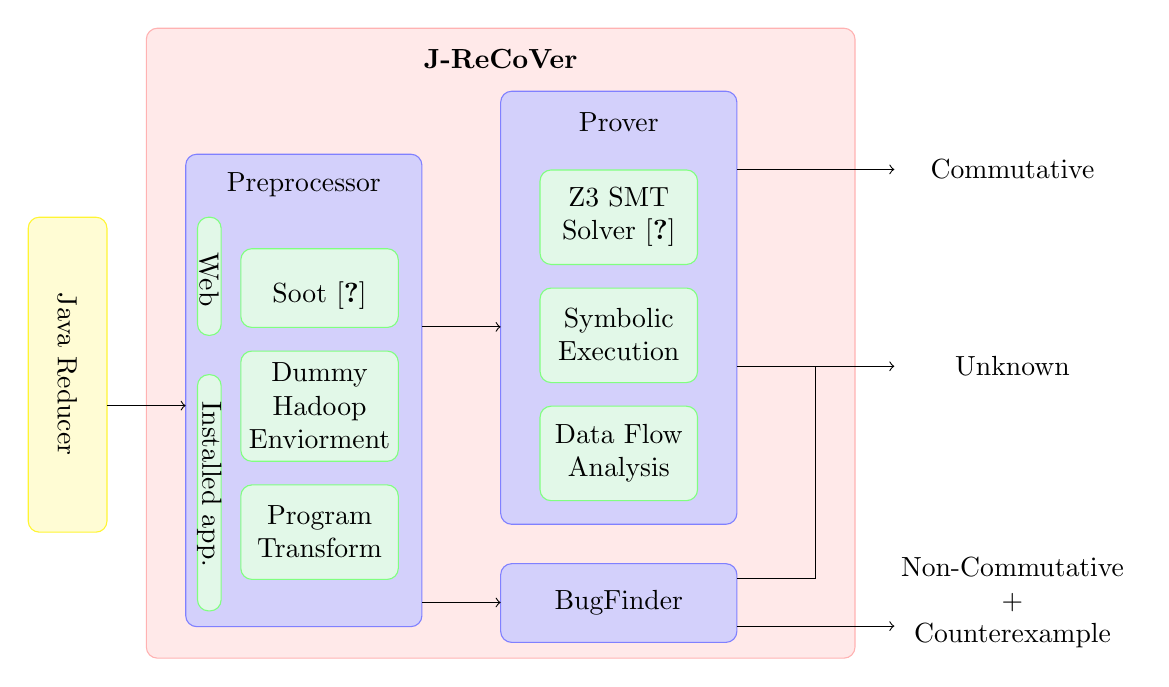
\begin{tikzpicture}
		

		%J-ReCoVer
		\node[draw=red!30, inner sep=0, anchor=north,rounded corners, fill opacity=0.85,text width=9cm,fill=red!10,minimum height=8cm] (jrecover) at (5.5,0.8) {};		
		\node at (5.5,0.4) {\textbf{J-ReCoVer}};

		%JAVA reducer
		\node[draw=yellow!80, inner sep=0, anchor=north,rounded corners, fill opacity=0.85,text width=1cm,fill=yellow!20,minimum height=4cm] (reducer) at (0,-1.6) {};
		\node[rotate=270, align = center] at (0,-3.6) {Java Reducer};
		
		
		%JPreprocessor
		\node[draw=blue!50, inner sep=0, anchor=north,rounded corners, fill opacity=0.85,text width=3cm,fill=blue!20,minimum height=6.cm] (preprocessor) at (3,-.8) {};
		\node[] at (3,-1.2) {Preprocessor};
		
		%JPreprocessor->Interface
		\node[draw=green!50, inner sep=0, anchor=north,rounded corners, fill opacity=0.85,text width=0.3cm,fill=green!10,minimum height=1.5cm] (interface1) at (1.8,-1.6) {};
		\node[rotate=270, align = center] at (1.8,-2.4) {Web};		
		
		\node[draw=green!50, inner sep=0, anchor=north,rounded corners, fill opacity=0.85,text width=0.3cm,fill=green!10,minimum height=3cm] (interace2) at (1.8,-3.6) {};
		\node[rotate=270, align = center] at (1.8,-5) {Installed app.};		
		
		%JPreprocessor->Technologies
		\node[draw=green!50, inner sep=0, anchor=north,rounded corners, fill opacity=0.85,text width=2cm,fill=green!10,minimum height=1cm] (soot) at (3.2,-2) {};
		\node at (3.2,-2.6) {Soot~\cite{soot}};		
		
		\node[draw=green!50, inner sep=0, anchor=north,rounded corners, fill opacity=0.85,text width=2cm,fill=green!10,minimum height=1.4cm] (symex) at (3.2,-3.3) {};
		\node at (3.2,-4) {
			\begin{minipage}[t]{0.222\textwidth}
			\centering
			Dummy\\ 
			Hadoop\\
			Enviorment
			\end{minipage}						
			};		
			
			\node[draw=green!50, inner sep=0, anchor=north,rounded corners, fill opacity=0.85,text width=2cm,fill=green!10,minimum height=1.2cm] (prog_trans) at (3.2,-5) {};
			\node at (3.2,-5.6) {
				\begin{minipage}[t]{0.222\textwidth}
				\centering
				Program\\ 
				Transform
				\end{minipage}						
			};				

		%JProver
		\node[draw=blue!50, inner sep=0, anchor=north,rounded corners, fill opacity=0.85,text width=3cm,fill=blue!20,minimum height=5.5cm] (prover) at (7,0) {};
		\node[] at (7,-0.4) {Prover};
		
		%JProver->Technologies
		\node[draw=green!50, inner sep=0, anchor=north,rounded corners, fill opacity=0.85,text width=2cm,fill=green!10,minimum height=1.2cm] (z3) at (7,-1) {};
		
		\node at (7,-1.6) {
			\begin{minipage}[t]{0.222\textwidth}
			\centering
			Z3 SMT \\
			Solver~\cite{z3}
			\end{minipage}						
		};		
		
		\node[draw=green!50, inner sep=0, anchor=north,rounded corners, fill opacity=0.85,text width=2cm,fill=green!10,minimum height=1.2cm] (z3) at (7,-2.5) {};
		
		\node at (7,-3.1) {
			\begin{minipage}[t]{0.222\textwidth}
			\centering
			Symbolic \\
			Execution
			\end{minipage}						
		};		
		
		\node[draw=green!50, inner sep=0, anchor=north,rounded corners, fill opacity=0.85,text width=2cm,fill=green!10,minimum height=1.2cm] (z3) at (7,-4.) {};
		
		\node at (7,-4.6) {
			\begin{minipage}[t]{0.222\textwidth}
			\centering
			Data Flow \\
			Analysis
			\end{minipage}						
		};		
		
		%JBugFinder
		\node[draw=blue!50, inner sep=0, anchor=north,rounded corners, fill opacity=0.85,text width=3cm,fill=blue!20,minimum height=1cm] (learner) at (7,-6) {};
		\node[] at (7,-6.5) {BugFinder};
				
				
		%JResults
		
		\node at (12,-1) {
			Commutative				
		};		
		
		\node at (12,-3.5) {
			Unknown					
		};		
		
		\node at (12,-6.5) {
			\begin{minipage}[t]{0.25\textwidth}
			\centering
			Non-Commutative	 \\
			+\\
			Counterexample
			\end{minipage}				
					
		};				
		
		
		\draw [->] (8.5,-6.8) -- (10.5,-6.8) ;	
		\draw [->] (8.5,-1) -- (10.5,-1) ;	
		\draw [-] (8.5,-6.2) -- (9.5,-6.2) --(9.5,-3.5);	
		\draw [->] (8.5,-3.5) -- (10.5,-3.5) ;	

		\draw [->] (4.5,-3) -- (5.5,-3) ;	
		\draw [->] (4.5,-6.5) -- (5.5,-6.5) ;	

		\draw [->] (0.5,-4) -- (1.5,-4) ;	
		
		\end{tikzpicture}
	}
	\caption{Overview of the J-ReCoVer Tool. }\label{fig:overview-jrecover}
\end{figure}


The Preprocessor component first compiles a reducer program to bytecode and use the tool Soot~\cite{soot} to convert it to the so called Jimple format, which is an intermediate language that is designed to make the analysis of Java program easier. Under the Hadoop MapReduce framework, the permutation of the input is caused by the scheduler/shuffler component and is affected by things like network latency, which is not controllable by the user. In order to handle this issue, we wrote our own dummy Hadoop interface for the reducer as a part of the Preprocessor component . So that the input/output of the reducer is now controlled by J-ReCoVer. Finally, we perform in the Preprocessor some simple program transformations that make the analysis easier. For example, we convert all output commands $out(e)$ inside loops to an special assignment $v_{out}:=e$.

In the Prover component, we reduce the commutativity problem to a SMT formula satisfiability problem, using the fact that all permutations of a list can be obtained by swapping consecutive elements finitely many times. At a high level, we check equivalence between a reducer program and its variant that have two consecutive inputs swapped. We show that this can be reduced to a simple SMT problem and give it to Z3~\cite{z3} for solving. In case that Z3 proved the formula unsatisfiable, J-ReCoVer stops and reports the reducer is commutative. 
If we run the approach in a naive manner, it does not scale to large programs and is very imprecise.  We will introduce two critical optimizations that makes the proposed approach works for real examples in Section~\ref{section:optimizations}: an improved symbolic execution algorithm to generate Z3 formulae and a data flow analysis to extract critical variables. More details of the algorithms used in the Preprocessor and the Prover components will be explained in Section~\ref{sec:preprocessor_prover} and the optimizations will be introduced in~\ref{section:optimizations}. 

The BugFinder component randomly generated 1500 pairs of list and its permutation for testing. A concrete counterexample is reported if inputting any pair of lists from the 1500 generated ones to the reducer generates different results.
Our procedure for generating random pairs is quite naive. We use five different input list of lengths 5, 7, 9 ,11, and 13. For each length, we generates 300 lists. For each list, we pick uniformly at random one of its permutations. Although the approach is simple, in practice it finds counterexamples in all of our non-commutative benchmarks.


\section{The Preprocessor and the Prover}
\label{sec:preprocessor_prover}

As mentioned, before entering the Prover components, the Preprocessor first performs a few program transformation to simplify the verification task. 
We assume the reducer $s_1;\rloop\{s_2\};s_3$ is given. We begin the section with our first program transformation task that handles the case when $s_2$ contains $out$ commands. The output of the first transformation task is a commutativity-equivalent reducer program where $out$ does not occur in $s_1$. Then we explain the algorithm of the Prover that works only in a special case where no read from input occurs in $s_1$. For general reducer programs, we introduce the second program transformation task whose output is a reducer program that contains all input/output behaviors of the original reducer (may contain behaviors not in the original reducer) and does not have $\cur$ in $s_1$, which can be analyzed by the algorithm of Prover.  

\subsection{The First Program Transformation Task in the Preprocessor}
\label{sec:program_trans1}
J-ReCoVer  first generates a new variable $v_{out_n}$ for the $n$-th output command $out(e)$ inside $s_2$ and replace the $out(e)$ command with an assignment $v_{out_n}:=e$. 
Notice that the value of $v_{out_n}$ stays the same from the point it has been assigned a value. 
If the values of $v_{out_n}$ are the same for all permutations of input lists at the end of $s_2$, we know that the a reducer that is commutative w.r.t. to all output commands inside the loop.

\subsection{The Prover: Reducing Commutativity to SMT Solving}
\label{sec:prover}
Below we begin with a simple version where $s_1$ never calls the $\cur$ function. Later we will explain how to handle the general case using program transformation. The command $s_2$ can be viewed as a function $F$ that reads the values of all variables and the current input before executing $s_2$ and outputs values of all variables after $s_2$. Formally, the function $F(n,x_1,x_2,\ldots,x_n): \Z^{n+1} \rightarrow \Z^n$ returns a tuple of values $x_1',x_2',\ldots,x_n'$, where $n$ is the current input value of the reducer, $x_i$ and $x_i'$ are the values of variables before and after the execution of $s_2$, respectively. The construction of $F$ from $s_2$ can be done in the standard way. We will introduce a more efficient data structure for the construction in Section~\ref{section:optimizations}.

We check if the formula is valid for all possible values of $n_1,n_2, x_1,x_2,\ldots,x_n$.
\begin{equation}
 F(n_1, F(n_2,x_1,x_2,\ldots,x_n) = F(n_2, F(n_1,x_1,x_2,\ldots,x_n) 
\label{eq:commu}
\end{equation}
The validity of formula~(\ref{eq:commu}) implies that swapping any two consecutive input values does not change the final variable valuation. Informally, it says that the values of all program variables stay the same when we execute the loop body twice (from any initial valuations of variables), one with the inputs $n_1$ and $n_2$ and the other with their reverse. That is, swapping any two consecutive input values does not change the output. 
Since any permutation of a sequence can be obtained by swapping consecutive values finitely many times~\cite{algebra}, this further implies that starting from the same variable valuation, the loop ends with the same valuation for any permutation of input values and produce the same sequence of output.

We show that this is sufficient to prove the commutativity of the reducer. Notice that $s_1$ does not read from the input and at $s_3$ all input has been read (this is the exit condition of the loop), both of them behave deterministically in the sense that from the same initial valuation, they output the same sequence of values and ends at the same valuation. From the validity of formula~(\ref{eq:commu}), any permutation of input values leads the reducer to the same valuation. Hence we know that any permutation of input values will produce the same sequence of output.

\subsection{The Second Program Transformation Task in the Preprocessor}
\label{sec:program_trans2}




\begin{figure}[t]
	\begin{minipage}{0.4\textwidth}
		\begin{algorithm}[H]
			$m := \cur + 10$; \;
			\Loop{}{
				\uIf{ $\cur > m$}{
					$m := \cur$ \;
				}
			};
			$out(m)$
		\end{algorithm}
		\caption*{(a)Reducer max$^+$}
	\end{minipage}
		\begin{minipage}{0.6\textwidth}
			\begin{algorithm}[H]
				$s:=*;$\;
				\Loop{}{
					\uIf{$s=1$}{$m := \cur + 10; s:= 2$}
					\uElseIf{ $\cur > m$}{
						$m := \cur$ \;
					}
				};
				$out(m)$
			\end{algorithm}
			\caption*{(b) Reducer max$^{+\mathtt{fix}}$}
		\end{minipage}
	\caption{Reducer examples}
	\label{fig:reducer_max}
\end{figure}




\begin{wrapfigure}{r}{0.56\textwidth} 
%		\vspace{-1.8cm}
		\begin{algorithm}[H]
			$s'_0;s:=*;$\;
			\Loop{}{
				\uIf{$s=1$}{ $x_{i_1} := \cur; s'_1; s:=2$}
				\uElseIf{ $s =2$}{ $x_{i_2} := \cur; s'_2; s:=3$}
				\uElseIf{ $s = 3$}{$\ldots$}
				\uElseIf{ $s = m$}{$x_{i_m} := \cur; s'_m; s:=m+1$}
				\uElse{ $s_2$}
			};$s_3$\;
		\end{algorithm}
		\caption{The second program transformation}
		\label{fig:general_program_transformation}
\end{wrapfigure} 
However, in reality, it is often that the $s_1$ part also reads from the input. See the example in Fig.~\ref{fig:reducer_max} (a), in this example, the program remembers the first input value in the variable $m$, increases its value by 10, and then updates its value to bigger ones if any occurs in the loop. The corresponding formula~(\ref{eq:commu}) is valid in this case, however, the reducer is not commutative. For example, the two lists $[1,2,3,4,5]$ and $[5,4,3,2,1]$ are permutations of each other, but the reducer respectively outputs $11$ and $15$ with them as the inputs. 

We handle the problem again by program transformation. For the example in Fig.~\ref{fig:reducer_max} (a), we move the prefix $s_1$ into the loop body and use a new variable $s$ to force that $s_1$ is always executed before the original loop body. The result after the transformation can be found in Fig.~\ref{fig:reducer_max} (b). Observe that the new reducer program over-approximates all possible inputs/outputs of the original one.
It also satisfies all assumptions required for the Prover: (I) $s'_0$ does not have any $\cur$ expression and (II) each branch (recall that this is defined in Section~\ref{section:integer-reducers}) of the loop body has at most one $\cur$. So we can apply equation~(\ref{eq:commu}) to prove its commutativity.
Since the new reducer has all the possible output of the original one, the new reducer is commutative implying that the original one is also commutative. 

For the general case, we first rewrite the $s_1$ part of the reducer $s_1;\rloop\{s_2\};s_3$ to the form 
$$s'_0;x_{i_1}{:=} \cur;s'_1.\ldots x_{i_{m}}{:=}\cur;s'_m, $$ where $\cur$ never occur in $s'_0,s'_1,\ldots, s'_m$. The reducer in Fig.~\ref{fig:general_program_transformation} is an over-approximation of the original reducer that satisfies all assumptions required for the Prover. Hence the equation~(\ref{eq:commu}) can then be applied to prove its commutativity.

\subsection{Limitations and assumptions}
At the back-end, we use SMT theory of integer arithmetics as the reasoning tool. In this implementation, we do not handle more advanced data-types such as string and floating point. 
The problem of variable overflow is not handled by this tool. In fact, if we consider all possible inputs of a reducer, almost all reducer programs will run into the problem of overflow. Even the basic example that computes the sum of all input values, overflow can occur when a list contains two maximal 64-bit integer values is used as the input. Nevertheless, such example might not be of the interests of MapReduce programmers, who usually care only about the data set they want to analyze. We are building another tool that estimates a safe bound of data size such that overflow will not occur. The programmer can than check if their data set fits the computed bound and use lager data type in the program when needed.

\section{Optimizations}
\label{section:optimizations}
In this section we explain how data flow analysis are used in our case to improve the precision of commutativity checking and the algorithm we used to construct the $F$ function in formula~(\ref{eq:commu}).

\subsection{Improving the precision of commutativity verification using data flow analysis}

We find that in many cases, formula~\ref{eq:commu} is a condition that is too strong for the reducer to be commutative. For instance, consider the example in Fig.~\ref{fig:reducer_opt}, in the loop body, the input is first stored in a variable $t$ and then added to $s$. In this case, the $F$ function returns the updated values of both $s$ and $t$ after the execution of loop body. Observe that 
$F(c_1, F(c_2,s,t) = (c_1+c_2, c_1)$ and $F(c_2, F(c_1,s,t) = (c_1+c_2, c_2)$, which follows that the corresponding equation~\ref{eq:commu} is invalid. The second component of the returned tuple, which corresponds to the value of $temp$ after executing the loop body twice, are $c_1$ and $c_2$, respectively. However, in this case, the value of $t$ is not important to the output of this reducer.

\begin{figure}[t]
	\begin{minipage}{0.4\textwidth}
		\begin{algorithm}[H]
			$s:= 0$; \;
			\Loop{}{
				$t:=\cur$;
				$s:= s + t$\;
			};
			$out(s)$\;
		\end{algorithm}
		\caption{A commutative reducer with an invalid equation~(\ref{eq:commu}).}
		\label{fig:reducer_opt}
	\end{minipage}
	\begin{minipage}{0.5\textwidth}
		\begin{algorithm}[H]
			$c_1;c_2;\ldots;c_i$\;
			\lIf{$g_1$}{$\ldots$}
			\lElseIf{ $g_2$}{$\ldots$}
			\lElseIf{ $g_3$}{$\ldots$}
			\lElseIf{ $g_m$}{$c_{i+1};\ldots ;c_n; out(v);\ldots$}
			\lElse{ $\ldots$}
		\end{algorithm}
		\caption{$out(v)$ in nested branches of $s_3$.}
		\label{fig:nested_out}
	\end{minipage}
\end{figure}




To handle such situation, we perform a simple data flow analysis to collect all variables whose value may propagate to the output after the loop. We do it in a backward manner.  With out loss of generality, we assume there is only one output command after the loop. Then the code after the loop (i.e., the $s_3$ part of the reducer) can only be in the form of Fig.~\ref{fig:nested_out}.
The commands $c_1\ldots c_n$ are either assignment commands $w:=e$ or branch command $\ite{g}{c'_1}{c'_2}$, and the only output command stays in the $m$-th layer of the branch command after $c_i$.

The data flow analysis algorithm works as follows.
A set $V_3$ whose value is initially a singleton set $\{v\}$ is used to remember important variables that might flow to the output commands in $s_3$.
The commands and guards will be inspected in the following order $c_{n}$,$\ldots$,$c_{i+1}$, $g_m$, $g_{m-1}$, $\ldots$, $g_1$, $s_i$, $\ldots$, $c_2$, $c_1$. For the case that a guard $g_j$ for $j\in [1,m]$ is being processed, we simply add all variables occurred in $g_j$ to $V_3$. 

Recall that the commands $c_j$ for $j\in [1,n]$ can only be in the form of $w:=e$ or $\ite{g}{c'_1}{c'_2}$.
For the case that $c_j$ is an assignment $w:=e$ and $w\in V_3$, we add all variables contained in $e$ to $V_3$. For the case that $c_j$ is an branch command $\ite{g}{c'_1}{c'_2}$, we process both $c'_1$ and $c'_2$ in a similar manner. Starting from the same set $V_3$,  after processing $c'_1$ and $c'_2$, we get respectively two sets $V_3^1$ and $V_3^2$, we take their union $V_3^1\cup V_3^2$ as the new value of $V_3$. 

Then we modify the equation~(\ref{eq:commu}) to the one below

\begin{equation}
F(n_1, F(n_2,x_1,x_2,\ldots,x_n) =_{V_2\cup V_3} F(n_2, F(n_1,x_1,x_2,\ldots,x_n) 
\label{eq:commu2}
\end{equation}
The special equality operator $=_{V_2\cup V_3}$ is defined (informally) as an equality that only focus on the positions of variables in $V_2\cup V_3$.
The set $V_2$ is defined as the set of variables we used to collect output values in the loop body $s_2$ of the reducer, i.e., $V_2= \{v_{out_k} \mid k \in [1,l]\}$, , where $l$ is the number of output commands occurred in $s_2$.

The use of equation~(\ref{eq:commu2}) is critical to the successful of our approach. In our evaluation, the ratio of examples that our approach can successfully analyze is significantly increased from $14\%$ to $98\%$. The details of the experiments can be found in Section~\ref{section:exp}.

\subsection{Computing the $F$ function using symbolic execution with efficiently data structure}
The computation of $F$ in equation~(\ref{eq:commu2}) can be done in several different ways. For example, one can construct a formula in the style of bounded model checking. Here we apply \emph{symbolic execution} to generate $F$. Our approach is very simple. First, we define the set $\Var_0=\{v_0 \mid v \in \Var \}\cup \{c_0\}$ as the set of initial symbolic values of all variables, where $c_0$ is used to denote the symbolic value from the input of the reducer.
A \emph{symbolic state} is a triple $\langle pc, val, cmds \rangle$, where the \emph{path condition} $pc$ is a guard in $\Grd$ over $\Var_0$, the \emph{symbolic valuation} is a mapping from variables in $\Var$ to an expression in $\Exp$ over $\Var_0$, and $cmds\in \Cmd$ is the remaining commands to be executed. The \emph{initial symbolic state} is $\langle \true, val_0, s_2\rangle$, where $val_0(v) = v_0$ for all $v\in\Var$. 
One can compute the next symbolic state of $\langle pc, val, c;cmds \rangle$ according to the following transition rules. Recall that $c$ is either in the form of $(v:= e_0)$ or $\ite{g}{c_1}{c_2}$:
\begin{enumerate}
	\item If $c$ is $(v:= e_0)$, the next symbolic state is $\langle pc, val[v \rightarrow e_0(val) ], cmds \rangle$.
	\item  If $c$ is $\ite{g}{c_1}{c_2}$, the next symbolic states are $\langle pc\wedge g, val, c_1.cmds \rangle$ and $\langle pc\wedge not\  g, val, c_2.cmds \rangle$. 
\end{enumerate}

Here $e_0(val)$ is a formula obtained by substituting every variable $v$ in $e_0$ with $val(v)$ and $val[v \rightarrow e_0(val) ]$ is obtained by reassigning the value of $v$ in $val$ to $e_0(val)$. The symbolic execution terminates when its path condition is conflict or the commands become empty. So far it is standard. 

For the loop body $s_2$, symbolic execution is guaranteed to terminate.
When the execution terminates, we collect all states with empty commands $\langle pc, val, \emptyset \rangle$ as a set $T$ and use them to create the function $F$ in formula~(\ref{eq:commu2}). 
First, we create for each variable $v\in\Var$ a formula $f_v$ whose initial value is $\false$. For each symbolic state $\langle pc, val, \emptyset \rangle \in Ts$, we reassign $f_v$ to $f_v \vee (pc \wedge val(v))$. 
Assuming that the set $P_2\cup P_3$ in equation~(\ref{eq:commu2}) equals $\{v_1,v_2,\ldots,v_n\}$, the function $F$ simply returns tuple $\{f_{v_1},f_{v_2},\ldots, f_{v_n}\}$.
 
However, doing symbolic execution in a naive way can be extremely inefficient. 
The length of the formula $val(v)$ can grow exponentially w.r.t. the input commands. For example, consider a simple command $u:=x+y;u:=u+u;u:=u+u$, each execution of $u:= u+ u$ will double the length of the expression storing the symbolic value of $u$. More concretely, after the execution of $u:=x+y$, the symbolic value of $u$ is $x_0+y_0$. After the two executions of $u:=u+u$, the value of $u$ changes to $x_0+y_0+x_0+y_0$ and $x_0+y_0+x_0+y_0+x_0+y_0+x_0+y_0$, respectively. One way to alleviate the problem is to apply some formula simplification algorithm, e.g., those build-in Z3~\cite{z3}. 
However, this will require some additional cost in the invocation of Z3. Here we propose in a very simple alternative solution that works quite well in our reducer benchmarks.

We use a more efficient data structure to store symbolic values. At a high level, in a symbolic state, we count the number of occurrences of each variables in $\Var_0$ and just update the count for operations such as $+$ and $-$. For other operations (e.g., $*$), we create the symbolic formula in the original way.
More concretely, we use a map $sv_x:\Exp\rightarrow \mathbb{N}$ (symbolic value of $x$) to remember the number of occurrences of each expression in $x$. Initially, $sv_x(x_0) = 1$ and $sv_x (e) =0$ for all $e\neq x$. Assume that the symbolic value of $x,y$ are $sv_x,sv_y$ in the current symbolic state. The symbolic value $sv'_x$ of $x$ after the assignment $x:=x\circ y$ is defined as follows. 

\begin{itemize}
	\item For the case that $\circ \in\{+,-\}$, we have $sv'_x(z) = sv_x(z)\circ  sv_y(z)$. 
	\item For the case that $\circ \notin\{+,-\}$, we compute an expression $e_1= (\Sigma_{z\in \dom{sv_x}} (z\times sv_x(z)) )\circ (\Sigma_{z\in \dom{sv_y}} (z\times sv_x(z)))$, where $\dom{sv}=\{e\mid sv(e)\neq 0\}$. Then we define $sv'_x(e_1) =1$ and $sv'_x(e_2) = 0$ for all $e_2\neq e_1$. 
\end{itemize}

This data structure is efficient for strong symbolic values of reducer programs mainly for reason that the operations $+$ and $-$ are quite heavily used in such programs. 



\section{Evaluation}
\label{section:exp}
J-ReCoVer is implemented in JAVA and build on top of the Soot~\cite{soot} 2.5.0 and Z3~\cite{z3} 4.7.1. We run J-Recover on a virtual machine running on a server with AMD Opteron 6376 CPU. 4GB of memory is allocated to this virtual machine. The operation system is Ubuntu 16.04.5 LTS. 


 In order to properly evaluate the performance of J-ReCoVer, we collect benchmark example from three different sources. 
First, we use the search engine \url{http://searchcode.com}~\cite{searchcode} to collect java programs contains the key strings ``public void reduce('' or ``protected void reduce(''.  Since there is an upper bound in number of returned results in the search engine, we add different search filters in order to get more data. We tried all $12$ combinations of $6$ code length filters $\{<50$, $ 50\sim 250$, $250\sim 450$, $450\sim 650$, $650\sim 850$, $850\sim 1050$, $1050\sim 1250\}$ 
and two filters for data sources $\{\url{github.com}, \url{bitbuckect.com}\}$. In total we get $11346$ Java programs. We then filter out cases that are not Hadoop MapReduce reducer programs (those do not import the Hadoop library, do not extend or implement the reducer interface) and obtain $1273$ examples. We further remove those that cannot be compiled, those that are identical to each other, or those uses non-numerical data types (e.g, string) and obtained $118$ programs as the final benchmark.
The second set of examples are those have been discussed in verification literatures~\cite{ChenHSW15,ChenSW16,SmithA16}. This set is relatively small, we have only $10$ examples. All benchmark examples can be found on the web-site of J-Recover.
For the third set of benchmarks, we created a program that randomly generate reducer program in order to test the scalability of J-Recover, which we can give as parameter a tuple $(N,B,A)$, where $N$ is the number of variables, $B$ is the branch statements, and $A$ is the number of assignment statement. All assignments are in the form of $v_1 := v_2\circ v_3,\circ\in\{+,-,\times\}$ and all guards are in the form of $v_1 \circ v_2, \circ\in\{\geq, >,=, \neq, <,\leq \}$.
 The source code of the random generator is available at \url{https://github.com/spencerwuwu/benchmark-generator}.

Our evaluation answers the following three questions:
\begin{itemize}
	\item Is J-Recover better than other competing tools/techniques?
	\item Are the two optimizations proposed in Section~\ref{section:optimizations} critical and effective?
	\item How good J-Recover scales?
\end{itemize} 

\subsection{Comparison with competing tools}
As already pointed out in~\cite{ChenHSW15}, reducer commutativity problems can be reduced to a reachability problem of programs. 
The examples in~\cite{ChenHSW15}, which includes \textsf{rangesum}\footnote{The sum of the second half of the input list.}, \textsf{avg}, \textsf{max}, \textsf{sep}\footnote{The number of occurrences of even numbers minus that of odd numbers.}, \textsf{sum}, are already included in SV-Comp~\cite{svcomp} (Software Verification Competition) benchmarks.
Although those examples are tiny and simple, none of the software verifiers are able to verify all of them according to the 2018 results, c.f., Table~\ref{tab:svcomp}. In this tools, the number of tools other than J-Recover are taken directly from the SV-Comp~\cite{svcomp} web-site. Although the machine we used are different, but the results of J-Recover will not be much different if we run it on other machines. 

\begin{table}
	\begin{tabular}{|l|l|l|l|l|l|l|}
\hline
		& \small CBMC\cite{cbmc2} 	& \small CPA-Seq\cite{cpachecker} & \small  ESBMC-kind\cite{esbmc} & \small  UAutomizer\cite{uautomizer} &\small  VeriAbs\cite{veriabs} &\small J-Recover\\
\hline
\hline
\small \textsf{rangesum}	& 0.96 	   & 30 		 & 2.2 				 &  10				 & 180       &9.9\\
\hline
\small \textsf{avg}			 &  TO      &  TO		  &  TO				 &  TO				 &  2          &10.9\\
\hline
\small \textsf{max}		    &  TO      &  TO		 &  TO				& TO				 &  7         &9.4\\
\hline
\small \textsf{sep}		     &  TO      &  TO		  &  TO				 & TO				 &  TO        &9.9\\
\hline
\small \textsf{sum}		    &  TO      &  TO		 &  TO				& TO				&  1.7       &9.9\\
\hline
	\end{tabular}
	\caption{SV-Comp 2018 results on reducer commutativity. For space reason, we only list results of tool with better performance in these examples, which includes top three tools in the overall ranking and the reachability safety category.}
	\label{tab:svcomp}
\end{table}




\subsection{The performance of J-Recover with and without optimizations}

\begin{table}
	\centering
	\begin{tabular}{|l|l|l|l|}
		\hline
		& &Equation~(\ref{eq:commu})	& Equation~(\ref{eq:commu2}) \\
		\hline
		\hline
		\multirow{3}{*}{Open repositories}&Commutative& 8&106\\ 
		\cline{2-4}
		&Non-commutative&9&9\\
		\cline{2-4}
		&Unknown&101&3\\
		\hline
		\hline
		\multirow{3}{*}{Literatures}&Commutative& 0&9\\
		\cline{2-4}
		&Non-commutative&1&1\\
		\cline{2-4}
		&Unknown&9&0\\
		\hline
	\end{tabular}
	\caption{The improvement of precision using data flow analysis.}
	\label{tab:opt1}
\end{table}


% Optimization table
\begin{table}
	\begin{tabular}{|l|l|l|l|l|l|l|}
\hline
		& \multicolumn{3}{c|}{\small w/o Optimization}	& \multicolumn{3}{c|}{\small Optimized} \\
\hline
		\small Lines & \small Average & \small Median & \small Timeout & \small Average & \small Median & \small Timeout \\
\hline
\hline
		50	&	11.104	&	10.446	&	0	&	10.284	&	10.193	&	0	\\
\hline                                                                              
		100	&	19.766	&	11.239	&	1	&	29.544	&	11.172	&	3	\\
\hline                                                                             
		150	&	88.741	&	17.943	&	12	&	63.931	&	13.984	&	7	\\
\hline                                                                             
		200	&	88.741	&	169.456	&	26	&	63.931	&	13.984	&	7	\\
\hline                                                                             
		250	&	232.348	&	300.000	&	43	&	175.976	&	248.998	&	30	\\
\hline
	\end{tabular}
	\caption{....}
	\label{tab:opt2}
\end{table}

% Optimization compare graph
\begin{tikzpicture}
	\begin{axis}[%
			xmin=-5, xmax=320,
			ymin=-5, ymax=320,
			xlabel=Optimize,
			ylabel=w/o Optimization
			]
	\addplot[scatter,only marks,%
		scatter src=explicit symbolic, mark=x]%
		file {plot_data/optimize.data};
\draw (-100,-100) -- (400, 400);
\end{axis}
\end{tikzpicture}

% BMC table
\begin{table}
	\begin{tabular}{|l|l|l|l|l|l|l|l|}
\hline
		& \multicolumn{3}{c|}{\small Optimized}	& & \multicolumn{3}{c|}{\small w/o Optimization} \\
\hline
		\small Lines/Vars & \small Average & \small Median & \small Timeout & Lines/Vars (jimple)& \small Average & \small Median & \small Timeout \\
\hline
\hline
		50/5	&	0.063	&	0.058	&	0	&	72.85/65.7	&	0.139	&	0.143	&	0	\\
\hline
		100/10	&	0.840	&	0.240	&	0	&	129.95/120.85	&	3.052	&	0.374	&	0	\\
\hline
		150/15	&	28.459	&	1.752	&	1	&	186.9/175.6	&	36.233	&	2.151	&	1	\\
\hline
		200/20	&	76.220	&	14.37	&	2	&	243.75/230.6	&	89.730	&	15.941	&	5	\\
\hline
		250/25	&	84.358	&	1.413	&	5	&	300.55/285.85	&	172.482	&	243.845	&	10	\\
\hline
	\end{tabular}
	\caption{....}
	\label{tab:opt2}
\end{table}

% BMC compare graph
\begin{tikzpicture}
	\begin{axis}[%
			xmin=-5, xmax=150,
			ymin=-5, ymax=150,
			xlabel=J-ReCoVer(s),
			ylabel=BMC(s)
			]
	\addplot[scatter,only marks,%
		scatter src=explicit symbolic, mark=x]%
		file {plot_data/bmc.data};
\draw (-100,-100) -- (400, 400);
\end{axis}
\end{tikzpicture}

%Discuss the tool’s practical capabilities with reference to the type and size of problems it can handle


\bibliographystyle{splncs-sorted}
\bibliography{refs}

\end{document}
